%This is the first chapter of the dissertation

%The following command starts your chapter. If you want different titles used in your ToC and at the top of the page throughout the chapter, you can specify those values here. Since Columbia doesn't want extra information in the headers and footers, the "Top of Page Title" value won't actually appear.

\chapter[][Recursive Jigsaw Reconstruction]{Recursive Jigsaw Reconstruction}

\textit{Recursive Jigsaw Reconstruction} (RJR) \cite{Jackson:2016mfb,ATLAS-CONF-2016-078} is a novel algorithm used for the analysis presented in this thesis.
RJR is the conceptual successor to the razor technique \cite{Rogan:2010kb,Buckley:2013kua}, which has been used successfully in many new physics searches \cite{SUSY-2014-05,SUSY-2014-06,CMS-SUS-13-004,CMS-SUS-12-005,CMS-SUS-11-024,SUSY-2011-22}.
In this chapter, we will first present the razor technique, and describe razor variables.
We will then present the RJR algorithm.
After the description of the algorithm, we will describe the precise RJR variables used by this thesis and attempt to provide some physical intuition of what they describe.

\section{Razor variables}

\subsection{Motivation}
In this thesis, we consider SUSY models where gluinos and squarks are pair-produced.
Pair-production is a consequence of the $R$-parity imposed in many SUSY models.
$R-$parity violation is highly constrained by limits on proton decay\todo{CitE}, and is often assumed in SUSY model building.
The Feynmann diagrams considered are shown in Fig.\ref{fig:feynmann_signal}.\todo{Check on W production thing, LO naming}.
\begin{figure}
\caption{Leading order Feynman diagrams for the SUSY signals considered in this thesis} \label{fig:feynmann_signal}
\subfloat[Disquark production]   {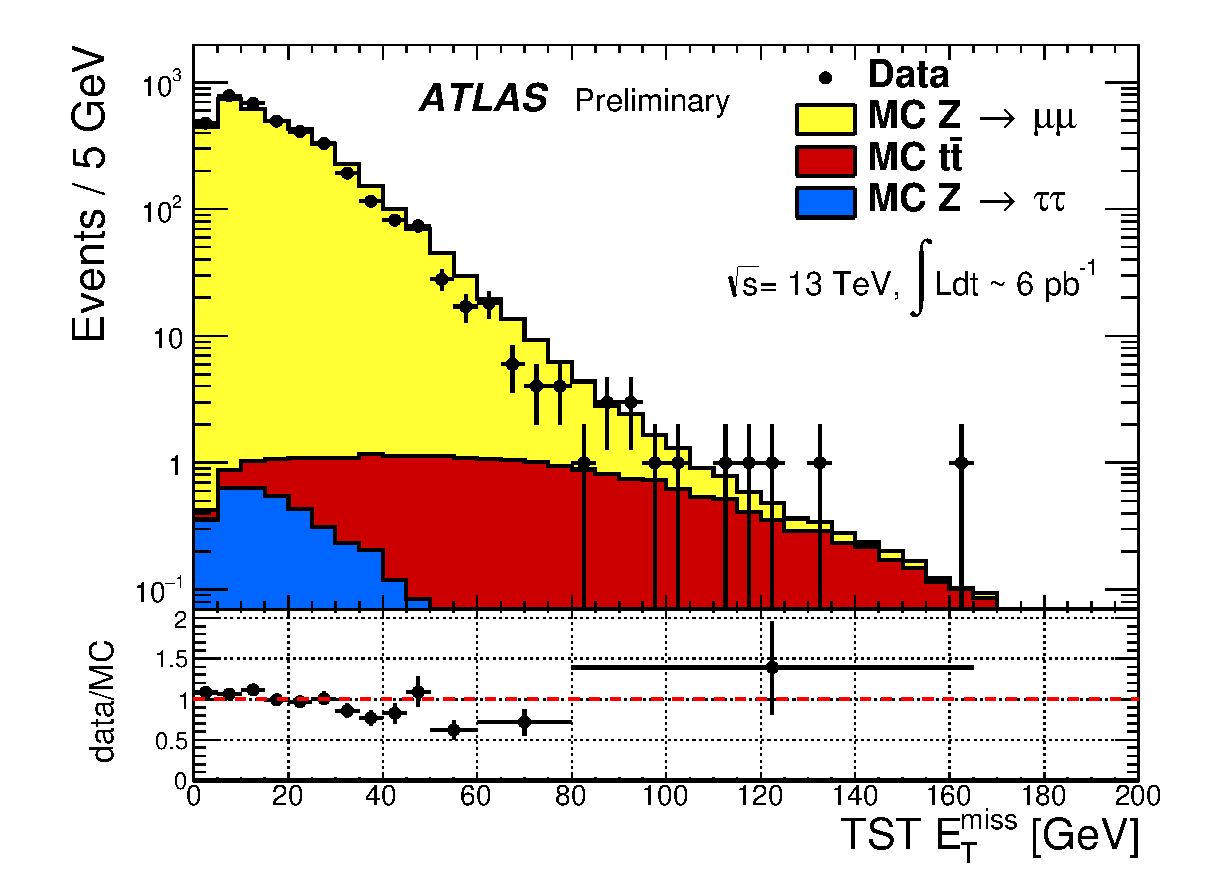
\includegraphics[width=.9\linewidth]{ATLAS-CONF-2016-078/fig_01a}}
\subfloat[Digluino production]   {\includegraphics[width=.9\linewidth]{ATLAS-CONF-2016-078/fig_01b}}
\subfloat[Digluino production with associated W bosons.]   {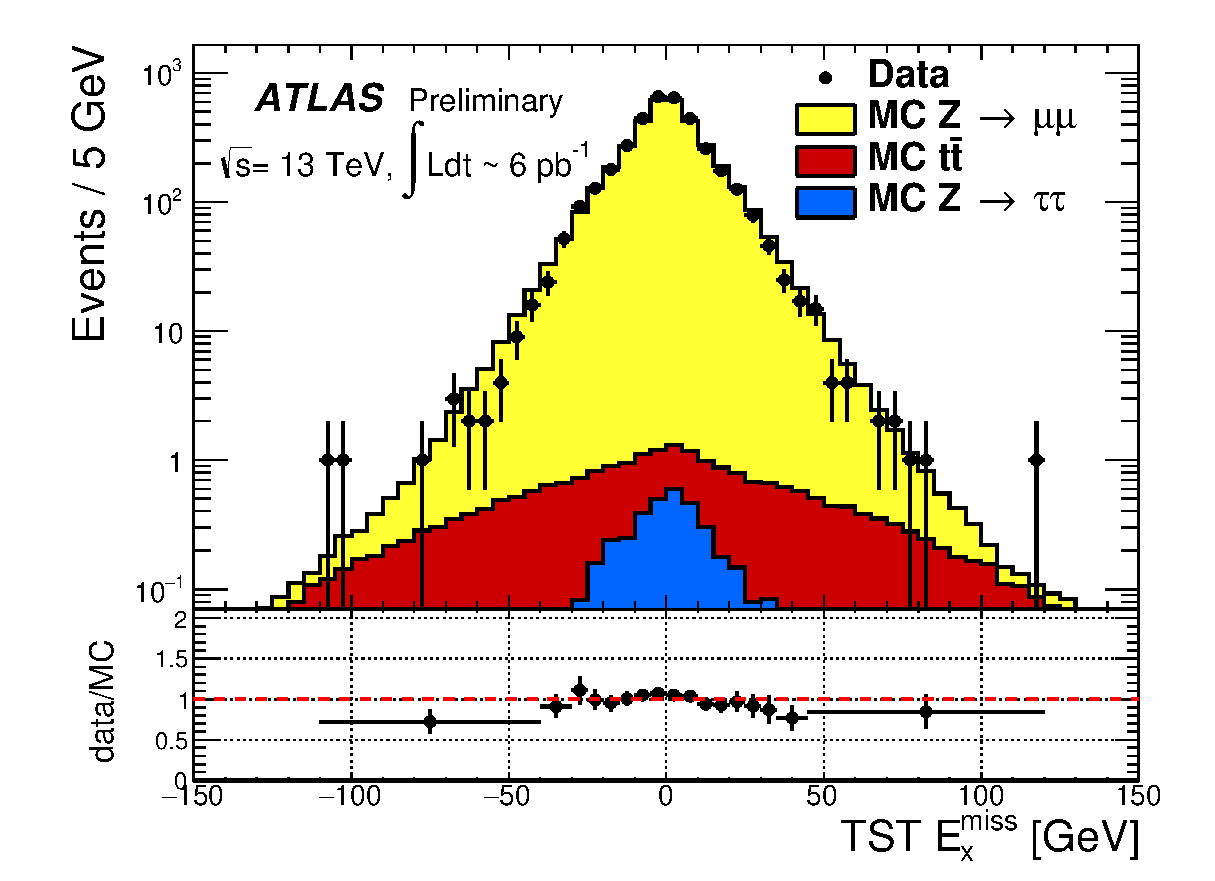
\includegraphics[width=.9\linewidth]{ATLAS-CONF-2016-078/fig_01c}}
\end{figure}

As discussed previously, the consequences of this $\mathbb{Z}_2$ symmetry are drastic.
To understand the utility of the razor variables, the stability of the lightest supersymmetric particle is very important.
In many SUSY models, including the ones considered in this thesis, this is the lightest neutralino \lsp.
This means that on either side of a SUSY decay process, where we begin with disparticle production, we have a final state particle which is not detected.
Generically, this leads to \met.
Selections based on \met are very good at reducing dominant backgrounds, for example from QCD backgrounds.

However, there are limitations to searches based on \met.
Due to jet mismeasurements, instrumental failures, finite detector acceptance, nongaussian tails in the detector response, and production of neutrinos inside of jets, there are many sources of ``fake'' \met which does not correspond to a Standard Model neutrino or new physics object such as an LSP.
An additional limitation is the complete lack of longitudinal information.
As events from i.e. QCD backgrounds tend to have higher boosts along the $z$-direction, this is ignoring an important handle in searches for new physics.
Finally, \met is only one object, which is a measurement for \textit{two} separate LSPs.
\todo{say somethign else here}
The \textit{razor variables} $(\mdr, R^2)$ are more robust than standard variables against these effects.

\subsection{Derivation of the razor variables}

To derive the razor variables $(\mdr, R^2)$, we start with a generic situation of the pair production of heavy sparticles with mass $\mheavy$.\footnotemark
\footnotetext{The razor variables have undergone confusing notational changes over the years.
We will be self-consistent, but the notation used here may be different from references.
}
Each sparticle decays to a number of observable objects (in this thesis, jets), and an unobservable \lsp of mass \mlsp.
We will combine all of the jets into a \textit{megajet}; this process will be described below.
We begin by analyzing the decay in the ``rough-approximation'', or in modern parlance, \textit{razor frame} (\rframe).
This is the frame where each sparticle is at rest.

In the \rframe, the decay is straightforward to analyze.
By construction, there are in fact two \rframe s, and they have identical kinematics.
Each megajet has energy $E_1^R, E_2^R$ in the frame of its parent sparticle, and we define a characteristic mass $M_R$:
\begin{align}
E_1^R &= E_2^R &= \frac{\mheavy^2 - \mlsp^2}{ 2 \mheavy } \\
M_R &= 2 \times E_1^R &= 2 \times E_2^R = \frac{\mheavy^2 - \mlsp^2}{\mheavy }.
\end{align}
For cases where $\mheavy >> \mlsp$, $M_R$ is an estimator of \mheavy.
This scenario happens in the SM, such as in \ttbar and \WW events, where the \lsp is instead a neutrino.

The question now is how to use this simple derivation in the lab frame, where we actually have measurements.
There are two related issues: how to combine the jets into the megajets, and how to ``transform'' to the \rframe.

To construct the megajets, the procedure is the following.
For a given set of jets $j_i, i = 0 , ... , n_{\mathrm{jet}}$, we construct \textit{all} combinations of their four-momenta such that there is at least one jet inside each megajet.
Among this set of possible megajets $\{J_{1,2}\}$, we make the following unique choice for the megajets.
We minimize the following quantity:
\begin{align}
m_{J_1}^2 + m_{J_2}^2.
\end{align}
In modern parlance, this is known as a \textit{jigsaw}.
It is important to note, this is a \textit{choice}.

We now describe how we translate our megajet kinematics, measured in the lab frame, to the \rframe.
This is a two-step procedure.
We perform two \textit{boosts}: a longitudinal boost $\beta_L$ and a transverse boost $\beta_T$.
Schematically,
\begin{align}
J_1^R &\xrightarrow[\beta_T]{}  J_1^{CM} &\xrightarrow[\beta_T]{} J_1^{\text{lab}} \\
J_2^R &\xrightarrow[-\beta_T]{} J_2^{CM} &\xrightarrow[\beta_T]{} J_2^{\text{lab}} \\
\end{align}
The $J_{1,2}^{\text{lab}}$ correspond directly to those in the megajet construction.
We drop the ``$\text{lab}$'' designation for the rest of the discussion.
The question is how to compute the magnitudes of these boosts, given the missing degrees of freedom.

For the transverse boost $\beta_T$, recall the two megajets have equal energies in their \rframe by construction.
This constraint can be reexpressed as a constraint on the magnitude of this boost, in terms of the boost velocity $\beta_L$ (and Lorentz factor $\gamma_L$):
\begin{align}
\beta_T = \frac{ \gamma_L (E_1^ - E_2) - \gamma_L \beta_L (p_{1,z} - p_{2,z})}
               { \hat{\beta}_T \cdot (\vec{p_{1,T}} - \vec{p_{2,T}} )}
\end{align}
where we have denoted the lab frame four-vectors as  $p_i = (E_i , \vec{p_{i,T}} , p_z)$.


\section{Recursive Jigsaw Reconstruction}


The algorithm proceeds by the imposition of a particular \textit{decay tree}, which corresponds to a simplified Feynmann diagram.
At each step in this decay tree, we can calculate variables of interest, through a series of simplifying assumptions.
In order to

\section{Variables used in the search for zero lepton SUSY}